Linear DC regulators are the most basic type of DC regulator and work by using a voltage reference and an error amplifier to control the output voltage. The output voltage is proportional to the input voltage, and the error amplifier compares the output voltage to the voltage reference to control the input current. Linear regulators are simple, but they are less efficient than other types of DC regulators and can generate significant heat.

Figure \ref{fig:linear_DC_regulator} has a implementation of linear DC regulator. 


\begin{figure}[]
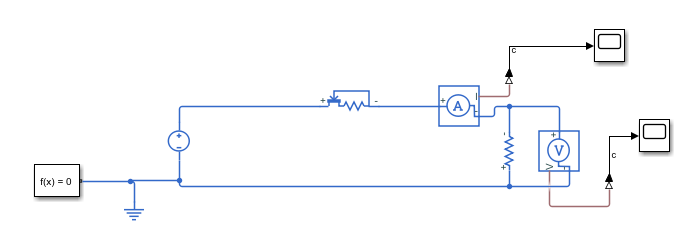
\includegraphics[width=\textwidth]{linear_DC_regulator.png}
\label{fig:linear_DC_regulator}
\caption{Matlab/simulink model of linear DC regulator}
\end{figure}



\begin{comment}

potential sources
https://en.wikipedia.org/wiki/Linear_regulator

\end{comment}